\documentclass[11pt]{article}

\usepackage{fullpage}
\usepackage{graphicx}
\usepackage{hyperref}

\title{Diabetes Prediction in Healthcare}
\author{Apurva Deshpande, Rushikesh Gholap, Sushmitha Rajeswari Muppa and Vedavarshita Nunna}
\date{} %don't display the current date

\begin{document}

\maketitle

\begin{abstract}

  As the prevalence of diabetes continues to rise globally, early prediction and intervention have become imperative for effective healthcare management. This research explores the application of machine learning classifiers to predict diabetes, aiming to identify the most accurate and robust approach. The study evaluates the performance of various individual classifiers, including Decision Trees, Logistic Regression, Naive Bayes, and K Nearest Neighbours, on a comprehensive dataset of health parameters. The research involves the analysis of a diverse range of features, such as age, body mass index, blood pressure, and cholesterol levels, to train and test the classifiers. Results indicate that individual classifiers exhibit varying degrees of accuracy, sensitivity, and specificity. To enhance predictive capabilities, an ensemble classifier is proposed, leveraging the strengths of multiple algorithms. The ensemble classifier is constructed through a systematic integration of individual classifiers, this type of ensembling is known as "Voting Ensemble" or "Majority Voting". The class that receives the most votes across the models is selected as the final prediction. The use of the mode function suggests that the ensembling strategy involves a simple majority voting scheme. The resulting accuracy is then calculated based on the ensemble predictions. The research evaluates the ensemble classifier's performance against other standalone classifiers, considering metrics such as precision, recall, F1-score. Furthermore, the study investigates the interpretability of the ensemble model, providing insights into the critical features contributing to diabetes prediction. This contributes to the understanding of the underlying factors influencing the disease and facilitates personalized healthcare strategies. In conclusion, this research highlights the importance of employing ensemble classifiers in diabetes prediction, showcasing their ability to enhance accuracy and reliability. The findings contribute valuable insights to the field of healthcare analytics, emphasizing the potential for machine learning to revolutionize early detection and intervention in diabetes, ultimately improving patient outcomes.
  
\end{abstract}

\section{Background and Related Work}

  Diabetes mellitus has emerged as a major global health concern, with an escalating prevalence that poses significant challenges to healthcare systems worldwide. The chronic nature of diabetes and its associated complications necessitate proactive and personalized healthcare strategies. Early prediction of diabetes is crucial for timely intervention, enabling healthcare providers to implement preventive measures and improve patient outcomes. Traditional methods of diabetes prediction often rely on clinical risk factors and demographic information. However, with the advent of machine learning techniques, there is an opportunity to harness the power of computational models to analyze complex datasets and extract valuable insights. Machine learning classifiers, such as Decision Trees, KNN, Naive Bayes, and Logistic Regression, have demonstrated promise in predicting diabetes based on diverse sets of health parameters.
  


The study on \textit{Diagnosis of Diabetes Mellitus Using Gradient Boosting Machine}\cite{paper1} explores applying Gradient Boosting for diabetes prediction. It combines weak models, like decision trees, iteratively correcting errors, contributing to the effectiveness of ensemble methods in diabetes diagnosis. In \textit{Performance enhancement of diabetes prediction by finding optimum K for KNN classifier with feature selection method,}\cite{paper2} the focus is on optimizing K-Nearest Neighbor (KNN) for diabetes prediction. The study explores finding the optimum K value and incorporates feature selection for accurate diabetes prognosis, providing insights into optimizing KNN for improved classification accuracy. The study \textit{Machine Learning Technique to Prognosis Diabetes Disease: Random Forest Classifier Approach}\cite{paper3} applies Random Forest Classifier for diabetes prognosis. This ensemble approach, using multiple decision trees, enhances predictive accuracy, emphasizing the potential of Random Forest Classifier as a robust forecasting model for diabetes. \textit{Nadeem et al.}\cite{paper4} introduce a fusion-based ML method for diabetes onset prediction, combining Support Vector Machines (SVM) and Artificial Neural Networks (ANN). Achieving a classification accuracy of 94.67\%, it surpasses other models, showcasing the effectiveness of combining SVM and ANN for diabetes prediction.

In summary, these studies collectively highlight the versatility of machine learning techniques in improving predictive models for diabetes mellitus, contributing to the ongoing advancement of predictive analytics in healthcare.

\section{Machine Learning Models}

% \begin{figure}[h]
% \begin{center}
% \includegraphics[scale=0.5]{Screenshot_-_030714_-_00_15_04.png}
% \end{center}
% \caption{This picture shows the Pyrobot playing field after a sample trial has just begun. Both robots have already begun to leave their respective bases and move toward the flag, coded as a light source in Pyrobot. The robots have access to their front sonar and light-detection sensor values, as well as 8 other inputs.}
% \label{setup}
% \end{figure}

\subsection{Decision Trees}
Decision Trees are hierarchical structures systematically navigate health parameters, such as age, BMI, and blood pressure, to classify individuals into diabetic or non-diabetic categories. Decision Trees inherently capture complex relationships, offering transparency and interpretability crucial for medical contexts. Their ability to handle non-linear interactions makes them effective in discerning patterns within diverse datasets. This research leverages Decision Trees to unravel key features influencing diabetes, contributing valuable insights for early prediction and tailored healthcare strategies.
Hence, they are utilized to shift through extensive datasets employing decision rules, efficiently categorizing data. This research explores diverse decision-tree-based techniques for data classification, as depicted in Figure 1. For instance, as indicated the decision tree checks blood glucose level, age, history of heart disease, body mass index and then decides if the sample is diabetes positive or not.


\subsection{Naive Bayes}
Naive Bayes is a probabilistic machine learning algorithm commonly used in healthcare and various other fields for classification tasks. It's based on Bayes' theorem, which calculates the probability of a particular event occurring given the presence of certain features. Despite its simplicity, Naive Bayes demonstrates remarkable efficiency in classification tasks by assuming independence among features, hence the "naive" assumption. In healthcare contexts, this algorithm efficiently categorizes individuals into diabetic or non-diabetic groups by considering various health parameters like age, BMI, blood pressure, and other relevant factors. Its simplicity and computational efficiency make Naive Bayes particularly suitable for large datasets. Although the assumption of feature independence might not always hold true in complex healthcare data, Naive Bayes still proves to be a robust and effective tool for preliminary analysis and classification tasks, offering valuable insights into disease prediction and patient stratification.

\subsection{K-Nearest Neighbors}
K-Nearest Neighbors (KNN) is a straightforward and intuitive machine learning algorithm utilized extensively in healthcare and various domains for classification tasks. KNN operates based on the principle of similarity, assigning classifications to data points by examining the majority class among their nearest neighbors. In healthcare scenarios, KNN could be employed to categorize individuals into diabetic or non-diabetic groups by assessing their similarity to other patients based on health parameters like age, BMI, blood pressure, and other relevant factors. This algorithm does not require explicit training and retains all the training data, making it particularly advantageous for smaller datasets. However, its computational intensity grows with the size of the dataset, impacting its efficiency for larger datasets. Despite its simplicity and susceptibility to outliers, KNN remains a valuable tool in healthcare for initial analysis and classification tasks, aiding in early disease prediction and patient grouping based on similarities in health metrics.

\subsection{Logistic Regression}
Logistic regression estimates the probability of an event occurring, based on a given dataset of independent variables. Since the outcome is a probability, the dependent variable is bounded between 0 and 1. In logistic regression, a logit transformation for linearizing sigmoid distributions of proportions is applied on the odds, such that, the probability of success is divided by the probability of failure. Logistic Regression is one of the most common classifiers for binary classification. It can also provide probability estimates, which can be useful in healthcare for assessing the likelihood of a patient having a particular condition. These probability estimates can be valuable in decision-making processes and risk assessment. Therefore in medicine, this analytics approach can be used to predict the likelihood of disease or illness for a given population. Healthcare organizations can set up preventative care for individuals that show higher propensity for specific illnesses. Also, since it is computationally efficient and easy to implement, making it easily accessible for healthcare practitioners and researchers without any extensive computational resources.
\begin{figure}[h]
\begin{center}
\fbox{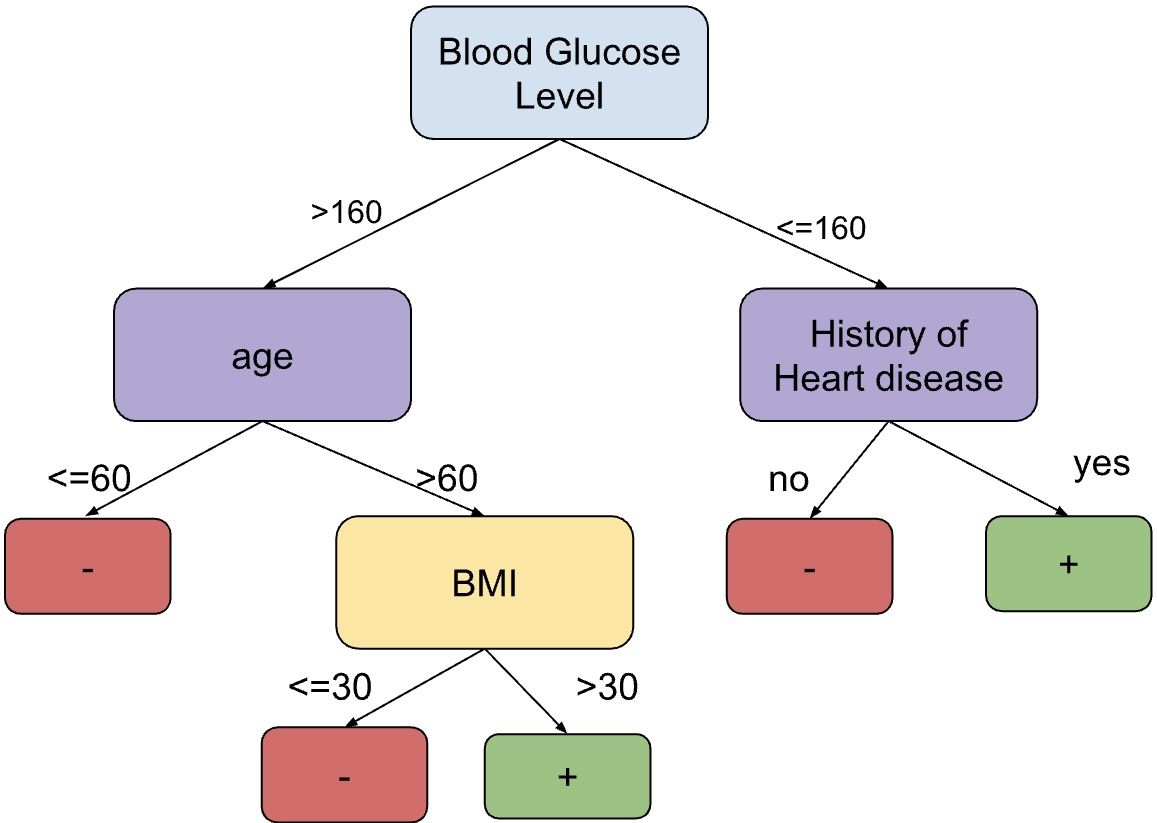
\includegraphics[scale=0.5]{dtree.jpeg}}
\end{center}
\caption{Decision Tree flowchart}
\label{experiment1fitness}
\end{figure}




\section{Evaluation of results}

Preceding model input, the dataset undergoes cleaning, and data values are normalized.  Random under-sampling for the majority class achieves a balanced dataset exceeding 20,000 rows. A 2:1 ratio splits the dataset into training and validation sets. Post-training, classifiers undergo evaluation through various metrics using the confusion matrix (Fig. 2). TP (true positive) signifies correctly predicted positive instances, TN (true negative) for negatives, FP (false positive) for incorrect positive predictions, and FN (false negative) for inaccuracies in negative predictions. Evaluation metrics encompass accuracy, sensitivity, specificity and Precision–Recall curve. Ensemble outperforms other diabetes models, attaining the highest accuracy (84.79\%), while Naive Bayes  demonstrates the lowest accuracy at 80.72\%. Nonetheless, accuracy alone is insufficient for comprehensive model assessment and prediction.


\begin{figure}[h]
\begin{center}
\fbox{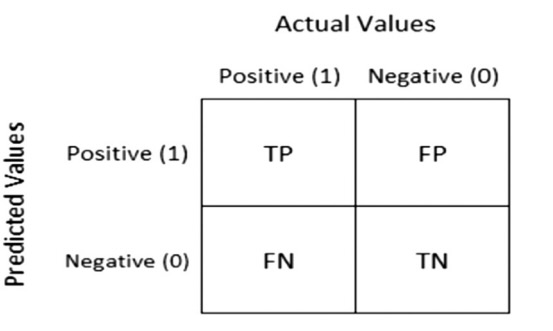
\includegraphics[scale=0.6]{cmat.jpeg}}
\fbox{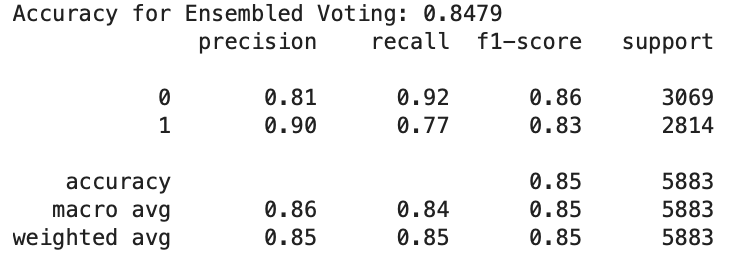
\includegraphics[scale=0.6]{imageEnsm.png}}
\end{center}
\caption{Confusion matrix and best classifier metrics}
\label{experiment1fitness}
\end{figure}

\begin{figure}[h]
\begin{center}
% \fbox{\includegraphics[scale=0.5]{image.png}}
\fbox{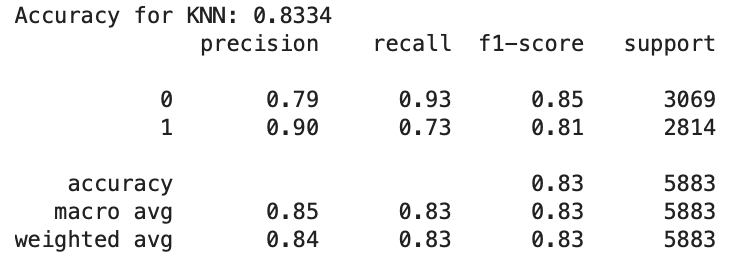
\includegraphics[scale=0.58]{imageKNN.png}}
\fbox{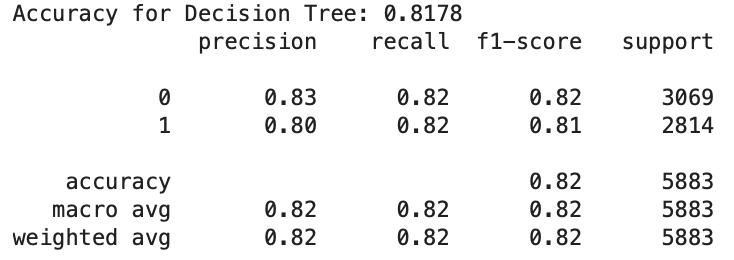
\includegraphics[scale=0.58]{imageDT.png}}
\fbox{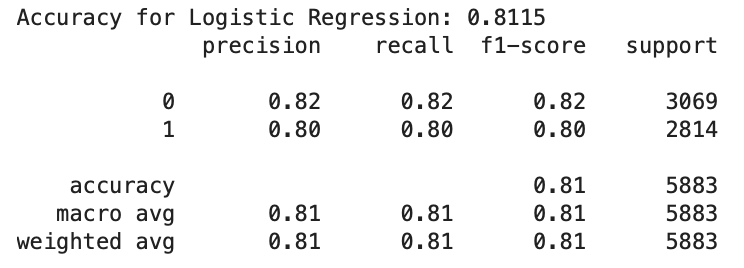
\includegraphics[scale=0.59]{imageLR.png}}
\fbox{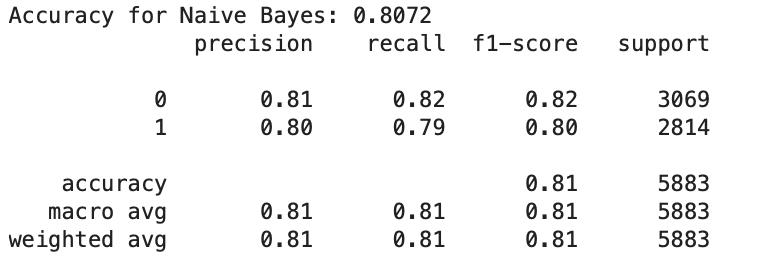
\includegraphics[scale=0.58]{imageNB.png}}
\end{center}
\caption{Classifier metrics}
\label{experiment1fitness}
\end{figure}

\begin{center}
\textbf{Precision = TP / (TP + FP)}
\end{center}

In the realm of disease detection, the prediction of false positives can result in misdiagnosis and the inefficient utilization of healthcare resources. Enhancing the precision of diagnostic models serves as a crucial solution to mitigate this issue. Precision specifically measures the accuracy of positive predictions, achieved by tallying correctly predicted positive samples (TP) and dividing by the total number of positive predictions (TP + FP), whether correct or incorrect. According to \textbf{Table 1}, among the evaluated classifiers, the Ensemble model exhibited the highest precision at 85\%, followed by KNN at 84\%, NB showed the least precision, registering a rate of 81\%.
\\ \\

\begin{center}
\textbf{Recall = TP / (TP + FN)}
\end{center}

Recall, also known as sensitivity, akin to precision, seeks to determine the proportion of accurately detected true positives. It achieves this by dividing the correctly predicted positive samples (TP) by the total number of positives, whether correctly or incorrectly predicted as positive (TP, FN). Recall assesses the number of accurately predicted positive instances out of all potential positive predictions. The highest sensitivity, or recall, is observed at 85\% for Ensemble, indicating that 85\% of diabetes cases in the test set were correctly identified by the Ensemble Voting classifier. NB and LR exhibits the poorest performance in this regard, with a recall rate of 81\%. Avoiding false negatives is crucial, as overlooking the presence of the disease can lead to delayed treatment and real harm.



\begin{center}
\textbf{F-measure = 2(Precision x Recall) / (Precision + Recall)}
\end{center}

\begin{figure}[h]
\begin{center}
\fbox{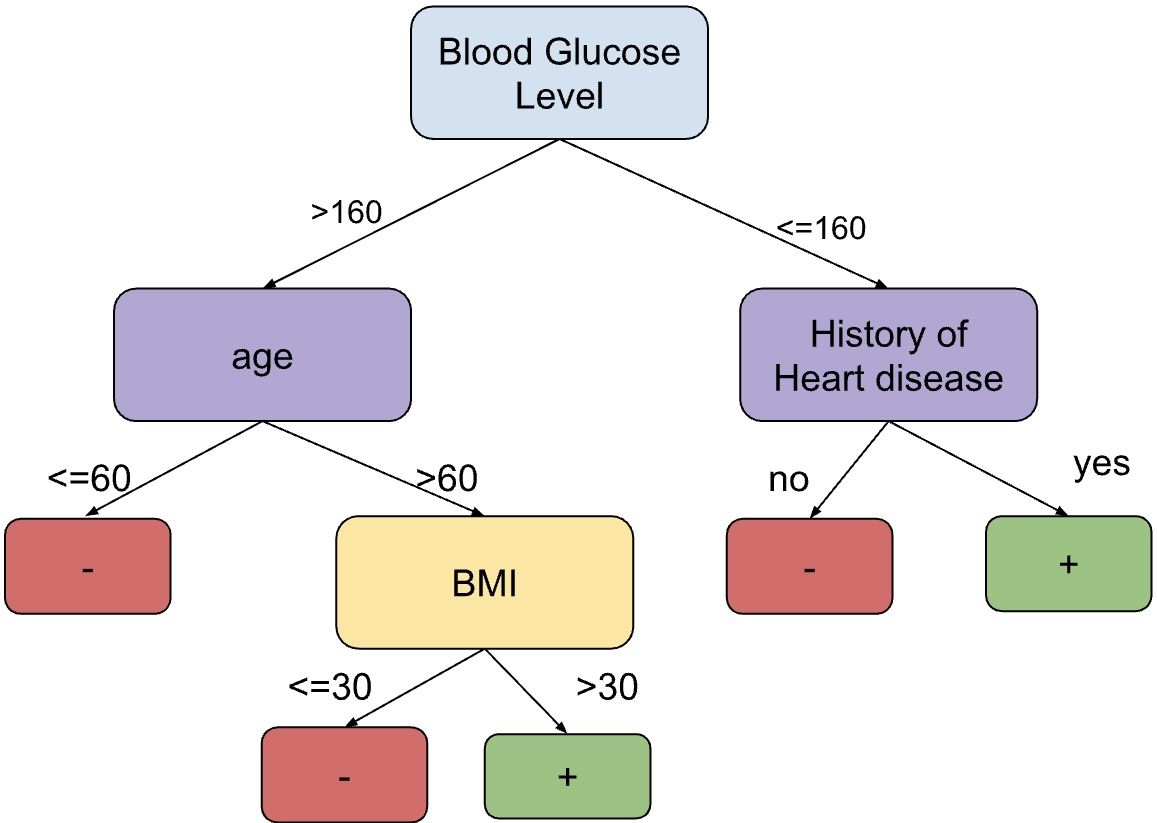
\includegraphics[scale=0.5]{dtree.jpeg}}
\end{center}
\caption{Decision Tree flowchart}
\label{experiment1fitness}
\end{figure}

\begin{figure}
    \centering
    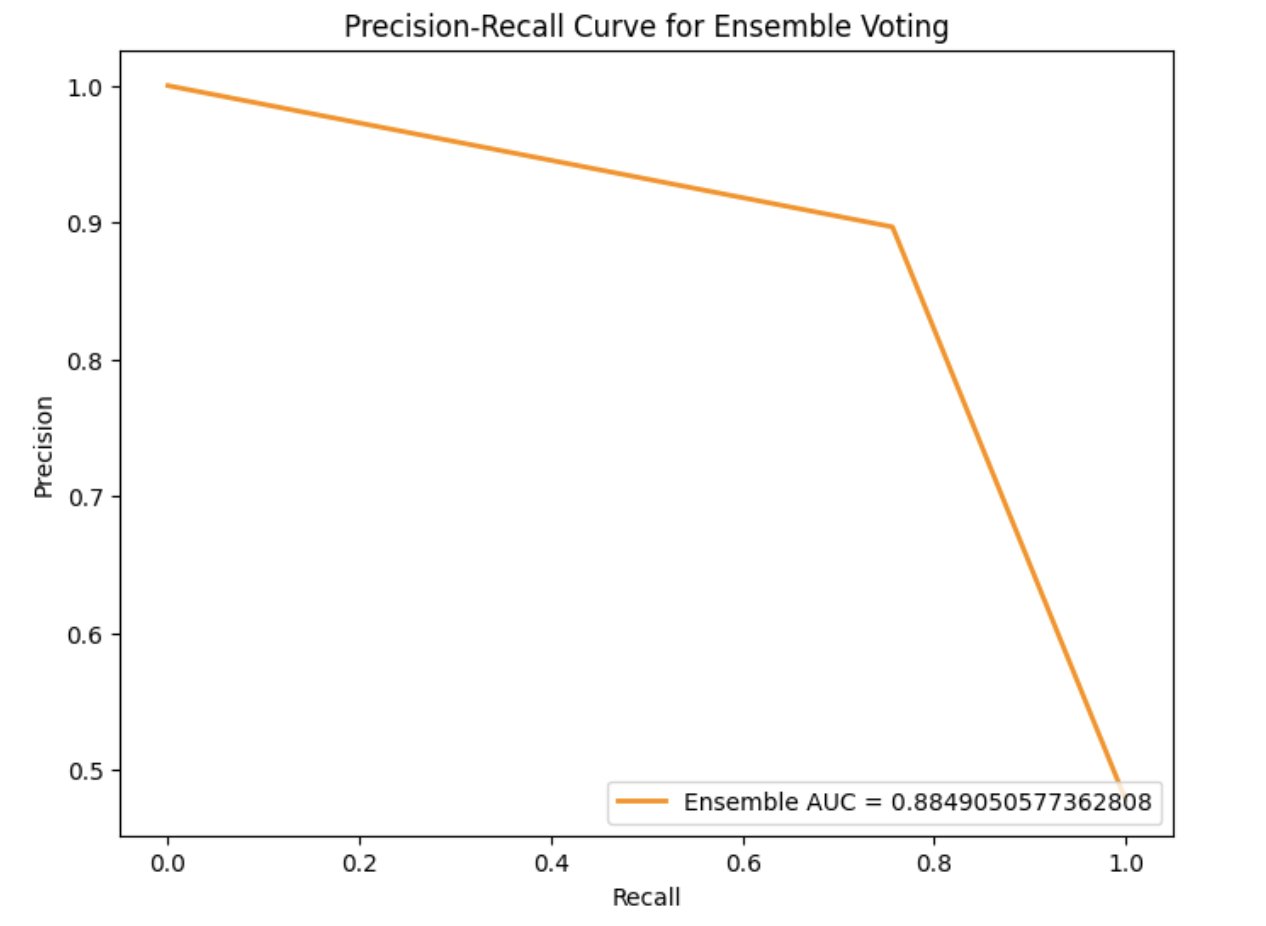
\includegraphics[width=0.5\linewidth]{imageAUC.png}
    \caption{Precision-Recall Curve}
    \label{fig:enter-label}
\end{figure}


A robust diabetes detection system needs to minimize both missed diagnoses and misdiagnoses. However, accuracy and specificity often present conflicting performance metrics. The F-measure takes into account both precision and recall, ranging from 0 to 1. A maximum value of 1 indicates perfect precision and recall, while a minimum value of 0 suggests that either precision or recall is zero. Ensemble attains the highest F1 score at 85\%, showcasing superior performance across all evaluation metrics. This substantiates Ensemble as the most effective classifier for diabetes in this study.

\section{Analysis and Conclusions}
Our research's primary contribution lies in creating machine learning predictive models for early diabetes detection. We investigated four classifiers (DT, KNN, LR, and NB) to predict diabetes likelihood, with the Ensemble classifier achieving the highest accuracy at 85\%. The study focused on evaluating diabetes prediction using crucial features. Leveraging the advanced classification capabilities of machine learning algorithms, our model holds substantial potential to assist medical practitioners significantly in the diagnosis process.

\begin{figure}[h]
\begin{center}
\fbox{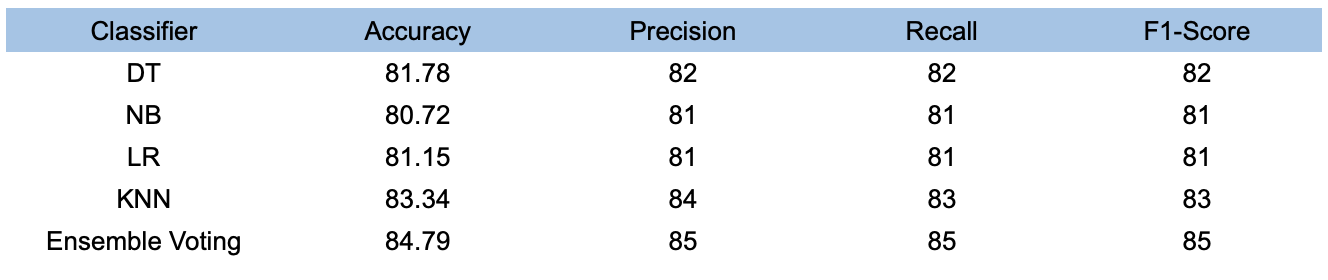
\includegraphics[scale=0.5]{AccTb.png}}
\end{center}
\caption{Classifier metrics}
\label{experiment1fitness}
\end{figure}

\begin{figure}[h]
\begin{center}
\fbox{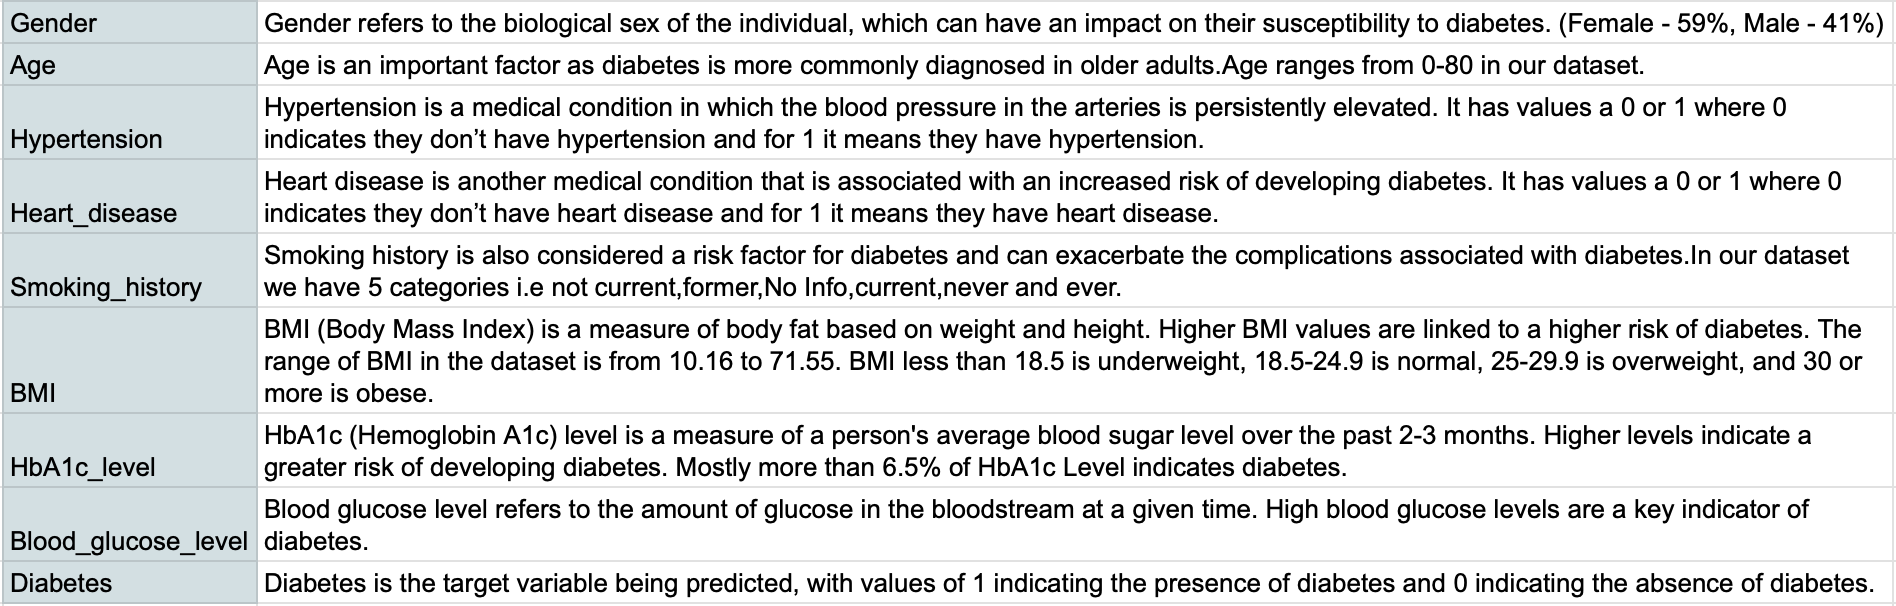
\includegraphics[scale=0.5]{imageDataset.png}}
\end{center}
\caption{DataSet}
\label{experiment1fitness}
\end{figure}


Ensemble voting, a robust technique in machine learning, has been applied to enhance the predictive performance of models in the context of diabetics prediction datasets. In the pursuit of refining diagnostic accuracy, multiple diverse models were employed to generate individual predictions. Subsequently, the ensemble voting methodology amalgamated these individual predictions, harnessing the collective intelligence embedded within the diverse model architectures. The fusion of distinct predictive perspectives not only serves to mitigate the impact of individual model idiosyncrasies but also capitalizes on the inherent diversity to achieve a more robust and generalized predictive outcome. Through the utilization of ensemble voting, this research endeavors to harness the strengths of various models, ultimately culminating in a consolidated prediction mechanism that excels in its ability to discern patterns and nuances within the intricate landscape of diabetics prediction. 



\section{Future Work}

Incorporating temporal analysis into the study involves a comprehensive exploration of how the predictive performance of the models evolves over time. This approach recognizes the dynamic nature of healthcare data, especially in the context of diabetes prediction. By scrutinizing temporal trends, one can discern patterns, fluctuations, and potential variations in predictive accuracy. Investigating whether the models adapt effectively to evolving trends becomes pivotal in understanding their long-term efficacy. This temporal consideration not only enhances the models' ability to capture nuanced changes in health parameters but also provides insights into their robustness for continuous and real-world applications. This approach aligns with the evolving nature of healthcare data, ensuring that predictive models remain relevant and effective in addressing the dynamic landscape of diabetes prevalence and risk factors over extended periods. Ultimately, incorporating temporal aspects enriches the models' adaptability, contributing to their sustained accuracy and utility in healthcare decision-making.

\begin{thebibliography}{1}

  \bibitem{paper1} Diagnosis of Diabetes Mellitus Using Gradient Boosting Machine \url{https://www.mdpi.com/2075-4418/11/9/1714}
  \bibitem{paper2} Performance enhancement of diabetes prediction by finding optimum K for KNN classifier with feature selection method \url{https://ieeexplore.ieee.org/abstract/document/9214129}
  \bibitem{paper3} Machine Learning Technique to Prognosis Diabetes Disease: Random Forest Classifier Approach \url{https://link.springer.com/chapter/10.1007/978-981-16-2164-2_19}
  \bibitem{paper4} An assessment of machine learning models and algorithms for early prediction and diagnosis of diabetes using health indicators \url{https://www.sciencedirect.com/science/article/pii/S2772442522000582#b7}
  



  \end{thebibliography}

\end{document}
